\documentclass[conference]{IEEEtran}

% ============================================================
% Packages
% ============================================================
\usepackage{cite}
\usepackage{amsmath,amssymb,amsfonts}
\usepackage{algorithm}
\usepackage{algorithmic}
\usepackage{graphicx}
\usepackage{textcomp}
\usepackage{xcolor}
\usepackage{booktabs}
\usepackage{multirow}
\usepackage{siunitx}
\usepackage{hyperref}
\usepackage{pifont}
\usepackage[caption=false,font=footnotesize]{subfig}

% 支持中文排版 (推荐在 Overleaf 中使用 XeLaTeX 编译)
\usepackage[UTF8]{ctex}

% Checkmark and crossmark
\newcommand{\cmark}{\ding{51}}
\newcommand{\xmark}{\ding{55}}

% ============================================================
% Title
% ============================================================
\title{PA-LOI: 基于潜在遮挡推断的主动预判，保障鬼探头场景下的自动驾驶安全}

\begin{document}
\maketitle

% ============================================================
% Abstract
% ============================================================
\begin{abstract}
鬼探头场景——即行人突然从遮挡车辆后方出现——对自动驾驶系统构成了最严峻的安全挑战之一。传统的反应式自动紧急制动（AEB）系统仅在行人进入视野后才进行检测，在典型的城市行驶速度下，这往往留不出足够的制动距离。
在本文中，我们提出了 \textbf{PA-LOI}（基于潜在遮挡推断的主动预判，Proactive Anticipation via Latent Occlusion Inference）。这是一个模块化的风险感知规划层，能够在检测到任何行人\emph{之前}，主动降低车辆靠近遮挡区域时的速度。
通过在潜在遮挡区域周围构建动态风险场，PA-LOI 使得自车在到达危险点时速度大幅降低，从而极大地扩展了下游 AEB 系统的有效制动窗口。该框架被设计为一个即插即用的安全模块，并被整合到一个最先进的交互感知规划框架中进行了验证，而该框架原本缺乏对不可见几何区域的显式处理能力。
我们在源自 Argoverse 2 运动预测数据集的两个截然不同的鬼探头场景中评估了 PA-LOI：一个复杂的十字路口和一个停满车辆的直道。我们在多个触发距离下对比了四种系统配置。
在十字路口场景中，PA-LOI+AEB 在前保险杠间距仅为 \SI{2.05}{\meter} 时即可实现零碰撞，而仅使用 AEB 则需要 \SI{3.25}{\meter}（安全边界改善了 \textbf{37\%}）。在更具挑战性的高车速直道场景中，仅使用 AEB 在所有测试距离下均发生碰撞，而 PA-LOI+AEB 在仅 \SI{1.75}{\meter} 的距离内就实现了零碰撞，并将最坏情况下的撞击速度降低了 \textbf{71\%}（从 \SI{7.75}{\meter\per\second} 降至 \SI{2.26}{\meter\per\second}）。
\end{abstract}

\begin{IEEEkeywords}
Automatic Emergency Braking, Autonomous Driving, Ghost Probe, Occlusion-Aware Planning, Pedestrian Safety, Risk Field
\end{IEEEkeywords}

% ============================================================
% I. Introduction
% ============================================================
\section{引言 (Introduction)}

行人伤亡仍然是城市交通安全的首要问题。其中最危险的场景之一被称为\emph{鬼探头} (Ghost Probe)~\cite{euroncap2023}：行人突然从遮挡物（如停放的车辆或公交车）后方走出，直接进入驶来车辆的路径。在行人完全暴露之前，驾驶员和车载传感器都无法看到他们，这留给车辆避免碰撞的时间微乎其微。

现代自动紧急制动 (AEB) 系统在减少行人伤亡方面已证明具有显著效果~\cite{cicchino2022effects}。然而，AEB 本质上是\emph{反应式}的：它只能在检测到行人后才开始介入。在鬼探头场景中，从检测到碰撞的时间窗口通常短于物理刹车所需的距离，导致 AEB 显得无能为力。

我们发现导致这些场景中 AEB 失败的根本原因是：\textbf{自车到达遮挡区域时的速度过快}。如果车辆在行人出现时行驶得更慢，同样的 AEB 系统将拥有足够的制动距离来完全避免碰撞。

基于这一洞察，我们提出了 \textbf{PA-LOI} 框架，该框架能够：
\begin{enumerate}
    \item 识别规划路径上由静态障碍物（停放车辆、建筑物）造成的潜在遮挡区域；
    \item 构建一个\emph{幻影风险场} (Phantom Risk Field)，对看不见的行人从这些区域出现的可能性进行建模；
    \item 将该风险场集成到基于 iLQR 的轨迹优化器的代价函数中，促使车辆在接近遮挡物时提前主动减速。
\end{enumerate}

该技术的核心贡献并非取代 AEB，而是作为一个\emph{前置互补模块}。通过在到达潜在危险点之前管理车辆的速度曲线，它极大地扩展了 AEB 的有效工作包络线 (operating envelope)。

% ============================================================
% II. Related Work
% ============================================================
\section{相关工作 (Related Work)}

\subsection{行人的自动紧急制动 (AEB)}
旨在保护行人的 AEB 系统已得到了广泛研究。Euro NCAP（欧洲新车碰撞测试）通过车对行人测试协议对其进行了标准化，包括 CPNA（近端成人）和 CPNC（近端儿童）场景~\cite{euroncap2023}。这些协议评估了行人在可能被遮挡的情况下穿过车辆路径时的 AEB 性能。尽管 AEB 可显著降低撞击速度，但已有研究表明，遮挡导致的检测时间缩短会严重削弱 AEB 的效能~\cite{cicchino2022effects}。

\subsection{遮挡感知运动规划}
过去有多项研究尝试解决遮挡下的规划难题。责任敏感安全模型 (RSS)~\cite{shalev2017rss} 通过对隐藏道路使用者做出最坏情况假设，提供了形式化的安全保证。基于部分可观察马尔可夫决策过程 (POMDP) 的行为规划器~\cite{zhang2021pomdp} 将遮挡建模为部分可观测性，并优化策略以在安全性和通行效率之间取得平衡。其他方法则在遮挡区域引入虚拟交通参与者（幻影智能体），以此来引导规划决策~\cite{schratter2019occlusion}。

虽然这些最先进 (SOTA) 的方法非常有效，但它们通常会带来巨大的计算开销，或者需要对假设实体进行复杂的概率追踪。与此相反，PA-LOI 采用了一种不同的思路，直接将几何遮挡的风险足迹嵌入轨迹优化的代价函数中。这种连续的空间表示方法无需离散的智能体实例化，也免去了昂贵的概率采样，造就了一个计算极度高效的架构，非常容易部署并集成到现有的工业规划器中。

\subsection{风险场方法}
势场法和风险场法在运动规划中由来已久~\cite{khatib1986potential}。近年来的研究已将风险场应用于自动驾驶的避障和车道保持。PA-LOI 对这一范式进行了扩展，通过几何遮挡分析来加权每个隐藏区域的风险贡献，专门针对\emph{尚未被观测到}的区域构建了新型风险场。

% ============================================================
% III. System Architecture
% ============================================================
\section{系统架构 (System Architecture)}

\subsection{概述}
PA-LOI 系统作为常规 AEB 模块上游的独立主动安全层运行。该架构由三个组件构成（图~\ref{fig:architecture}）：

\begin{enumerate}
    \item \textbf{遮挡几何分析器}：识别遮挡对象并计算自车规划路径沿线的阴影区域。
    \item \textbf{动态风险场生成器}：围绕识别出的遮挡区域构建幻影风险走廊，风险强度与遮挡严重程度及距离成正比。
    \item \textbf{集成风险的轨迹优化器}：PA-LOI 对 MIND 规划器~\cite{mind2025}进行了扩展。MIND 是一款基于 iLQR 优化的先进多模态交互感知规划框架。尽管 MIND 擅长预测和应对能够观测到的交通流，但它本身缺乏对不可见区域的感知能力。PA-LOI 填补了这一空白，将风险场作为附加代项引入，生成在靠近遮挡时主动减速的轨迹。
\end{enumerate}

下游的 AEB 模块独立运行，当通过 TTC（碰撞时间）分析检测到物理碰撞威胁时，直接触发紧急制动。

\begin{figure}[htbp]
\centering
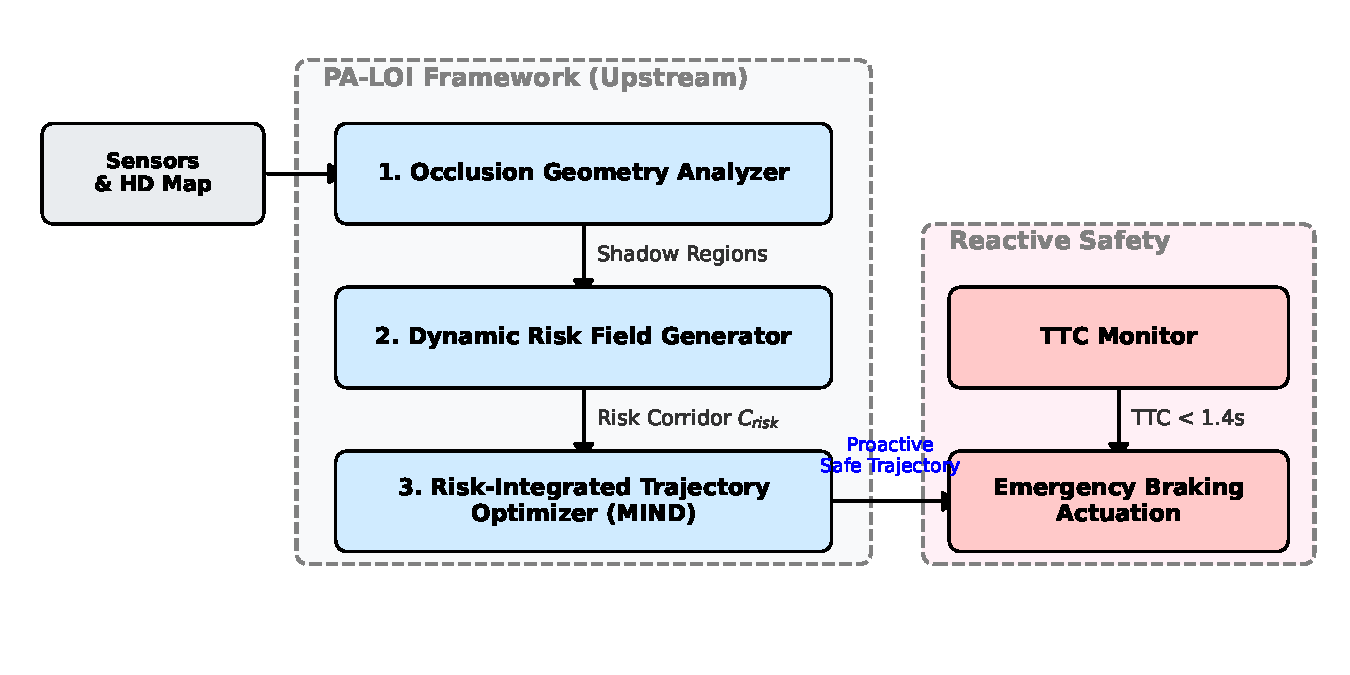
\includegraphics[width=\columnwidth]{figures/architecture.pdf}
\caption{PA-LOI 系统架构图。}
\label{fig:architecture}
\end{figure}

\subsection{动态风险走廊 (Dynamic Risk Corridor)}
当自车接近遮挡物（如停靠的公交车）时，PA-LOI 会以遮挡区域为中心构建一条\emph{动态风险走廊}。走廊参数定义如下：
\begin{align}
    d_{\text{critical}} &= d_{\text{vehicle}} + v_{\text{ego}} \cdot t_{\text{buffer}}, \label{eq:dcrit} \\
    d_{\text{outer}} &= \max(d_{\text{lane}}, d_{\text{critical}} + d_{\text{margin}}). \label{eq:douter}
\end{align}
其中 $d_{\text{vehicle}}$ 是车辆半宽，$v_{\text{ego}}$ 是当前自车速度，$t_{\text{buffer}}$ 是安全时间裕度，$d_{\text{lane}}$ 是车道半宽，$d_{\text{margin}}$（在我们的实验中设置为 \SI{0.5}{\meter}）提供了额外的侧向安全缓冲，确保走廊涵盖边缘情况下的车辆定位。至关重要的是，$t_{\text{buffer}}$ 经过精确校准，与下游 AEB 所采用的保守的 \SI{-4.0}{\meter\per\second\squared} 减速极限对齐，从而保证了在摩擦力下降的路况下仍能提供充足的物理制动包络。

轨迹 $\tau$ 穿过走廊的风险代价公式为：
\begin{equation}
    C_{\text{risk}}(\tau) = w_{\text{risk}} \sum_{t} \phi(d_{\text{lat}}(t), d_{\text{long}}(t)),
    \label{eq:risk_cost}
\end{equation}
其中 $\phi(\cdot)$ 是一项与距离相关的风险核函数，$w_{\text{risk}}$ 是可调风险权重。该风险场的生成逻辑在算法~\ref{alg:risk_field} 中进行了总结。

\begin{algorithm}[htbp]
\caption{动态风险场生成 (Dynamic Risk Field Generation)}
\label{alg:risk_field}
\begin{algorithmic}[1]
\REQUIRE 自车状态 $s_{\text{ego}}$, 地图 $\mathcal{M}$, 遮挡集合 $\mathcal{O}$
\ENSURE 风险代价场 $C_{\text{risk}}$
\FOR{每个遮挡 $o \in \mathcal{O}$}
    \IF{$\text{距离}(s_{\text{ego}}, o) < d_{\text{trigger\_zone}}$}
        \STATE 使用公式~\eqref{eq:dcrit} 计算 $d_{\text{critical}}$
        \STATE 使用公式~\eqref{eq:douter} 计算 $d_{\text{outer}}$
        \STATE $C_{\text{risk}} \gets C_{\text{risk}} + w_{\text{risk}} \cdot \phi(d_{\text{critical}}, d_{\text{outer}})$
    \ENDIF
\ENDFOR
\RETURN $C_{\text{risk}}$
\end{algorithmic}
\end{algorithm}

\subsection{AEB 模块}
AEB 模块执行基于 TTC 的紧急制动策略。一旦检测到障碍物低于临界 TTC 阈值（$T_{\text{critical}} = \SI{1.4}{\second}$），系统即施加 $a_{\text{max}} = \SI{-4.0}{\meter\per\second\squared}$ 的最大制动减速度。虽然现代 AEB 系统在干燥沥青路面上可以达到 \SI{-8.0}{\meter\per\second\squared}，但我们故意采用了 \SI{-4.0}{\meter\per\second\squared} 这样一个极其保守的极限，以模拟恶劣的路面摩擦条件（例如潮湿或湿滑的表面），避免乘客因极端冲击而受伤。这使得我们能够在最糟糕的物理约束下，观察系统的安全边界并衡量主动减速所带来的价值。一旦被触发，AEB 将保持持续制动，直到车辆完全停下，避免出现释放后再加速的危险振荡行为。

% ============================================================
% IV. Experimental Setup
% ============================================================
\section{实验设置 (Experimental Setup)}

\subsection{仿真环境}
我们的实验建立在 Argoverse 2 运动预测数据集的衍生场景上~\cite{argoverse2}，该数据集提供了真实的道路几何、周围的交通背景车辆以及高精地图信息。仿真实验的物理运行频率为 \SI{50}{\hertz}，规划计算频率为 \SI{10}{\hertz}。

\subsection{鬼探头测试场景选择}
为了全面评估 PA-LOI 规划器在严重遮挡下的安全性能，我们从 Argoverse 2 数据集中选取了两个截然不同的“零样本”(zero-shot) 测试场景（如图~\ref{fig:scenarios}）：
\begin{enumerate}
    \item \textbf{停满车辆的直道（泛化场景）}：如图~\ref{fig:scenarios}a 所示，自车在一条笔直的城市主干道上行驶，右手侧停放着一长排密集车辆。这道“视觉高墙”完全阻断了对人行道的视线。一名行人突然从一辆带有盲区的停靠车辆（图中标号 No.22153）前段窜出并横穿自车车道。该测试旨在检验系统对绵延不断的静态遮挡物保持连续防御姿态的能力。
    \item \textbf{存在静止交通流的复杂十字路口}：如图~\ref{fig:scenarios}b 所示，自车正在穿过一个繁忙的十字路口。右侧相邻车道上停着一列等待信号灯的车辆（标号 No.199599），造成了路口中心接近区域的严重遮挡。同样，一名行人从该静止车辆前侧冲出。这评估了系统在复杂拓扑结构中，处理排队交通造成的局部盲点能力。
\end{enumerate}

\begin{figure}[ht]
    \centering
    \subfloat[Straight road]{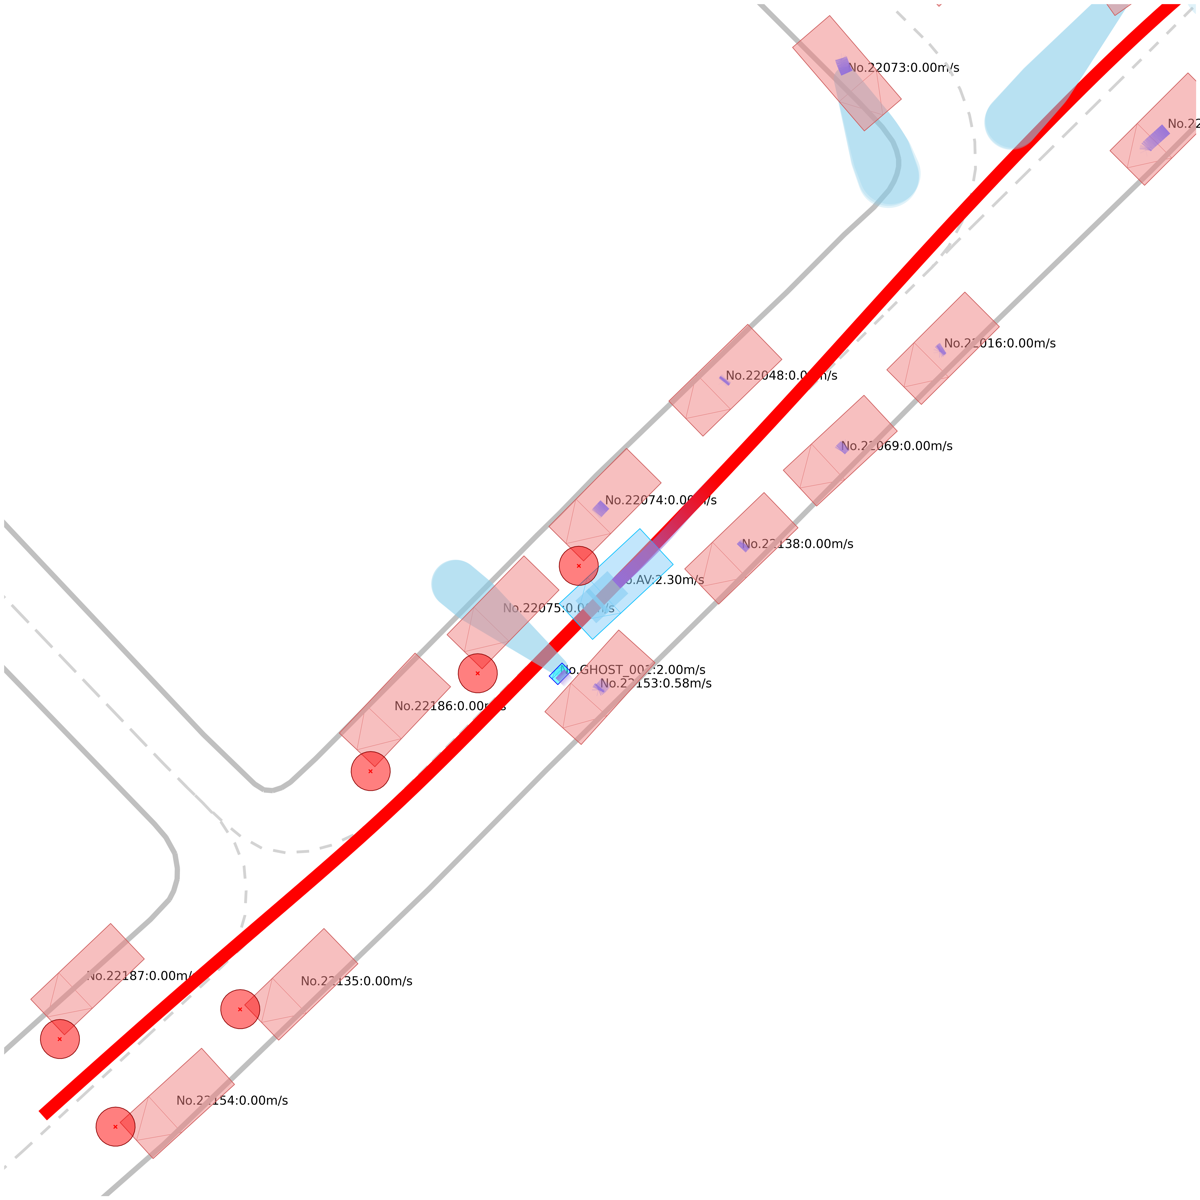
\includegraphics[width=0.48\columnwidth]{figures/straight_road.png}}
    \hfill
    \subfloat[Complex intersection]{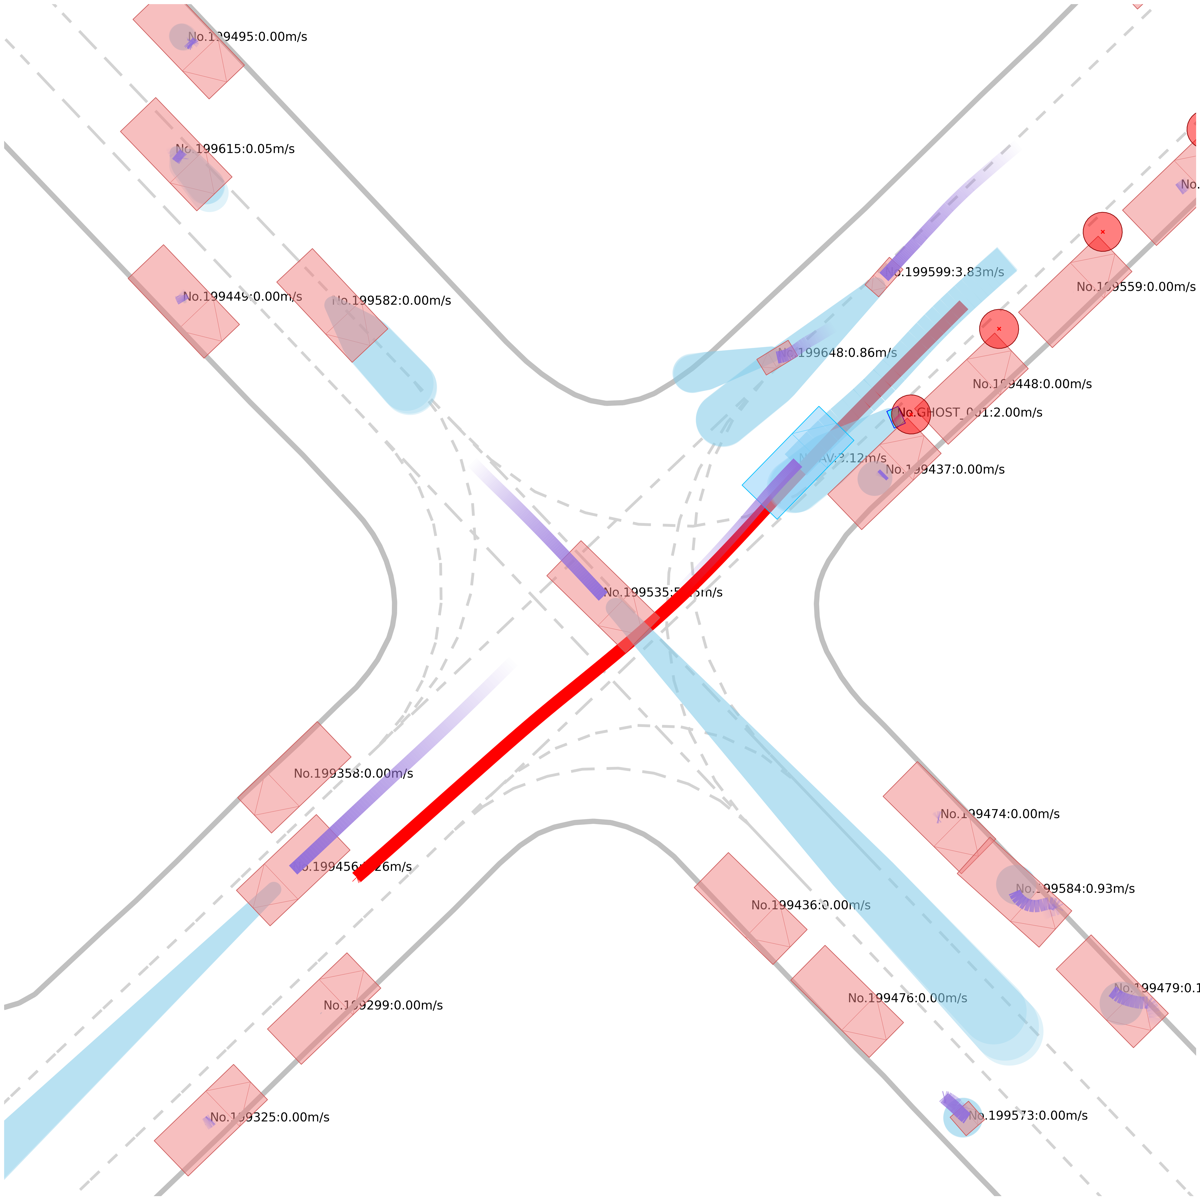
\includegraphics[width=0.48\columnwidth]{figures/intersection.png}}
    \caption{两种对抗性鬼探头测试场景概览。(a) 一条直道，路边密集的停车遮挡了正在过马路的行人。(b) 复杂的十字路口，停滞的车辆在中心交汇区形成了严重的局部视线盲区。}
    \label{fig:scenarios}
\end{figure}

两个场景均采用一套受 Euro NCAP CPNA 协议~\cite{euroncap2023} 启发的严格且确定性的触发机制。所谓的“幽灵行人”精确地在自车突破预定义的纵向碰撞触发距离 $d_{\text{trigger}}$ 时立刻产生。在十字路口场景中，$d_{\text{trigger}} \in \{3.0, 3.5, 4.0, 4.3, 4.5, 5.0, 5.5\}$ m（7 组数据）；而直道场景使用 $d_{\text{trigger}} \in \{3.0, 3.5, 4.0, 4.5, 5.0\}$ m（5 组数据）。自车前保险杠离行人的实际间距计算为 $d_{\text{bumper}} = d_{\text{trigger}} - \SI{2.25}{\meter}$（车辆半长）。触发后，行人立即以 \SI{2.0}{\meter\per\second} 的激进横向爆发速度，从 \SI{1.5}{\meter} 的距离切入并在车道正中心停止。这种标准化的伏击设计构成了一个绝对的对抗性几何灾难，保证了如果自车未能进行主动预判减速，事故将 100\% 发生。

\subsection{系统配置}
我们在完全相同的测试条件下对比了四种配置：
\begin{enumerate}
    \item \textbf{Vanilla MIND}：原始的基于 iLQR 的常规规划器，没有任何遮挡感知能力，也不开启 AEB。自车按照规划器自己更偏爱的高速曲线行驶。
    \item \textbf{AEB Only (对照组)}：没有遮挡感知的 MIND 规划器叠加了反应式 AEB 模块（$a_{\text{max}} = \SI{-4.0}{\meter\per\second\squared}$）。
    \item \textbf{PA-LOI + AEB}：集成了 PA-LOI 遮挡风险场的 MIND 规划器，同时叠加相同的 AEB 模块。
    \item \textbf{Conservative WCA}：最坏情况假设法 (WCA)。将其作为由于责任敏感安全 (RSS) 模型的极简化横纵向替代方案。它强行计算必须在不可见区域边界前无条件无伤停下的严格物理上限，以牺牲所有效率的代价将目标速度限制死，在数学上实现 0 碰撞防守。
\end{enumerate}

\subsection{评估指标}
\begin{itemize}
    \item \textbf{碰撞结果 (Collision occurrence)}：二元布尔结果（发生碰撞 / 安全停下）。
    \item \textbf{撞击速度 (Impact velocity, $v_{\text{imp}}$)}：发生碰撞时自车接触行人瞬间的残余速度 (\si{\meter\per\second})。
    \item \textbf{安全临界间距 (Safe critical distance)}：系统能够刚好实现零碰撞的最小允许 $d_{\text{bumper}}$。
\end{itemize}

% ============================================================
% V. Results
% ============================================================
\section{实验结果 (Experimental Results)}

\subsection{定量结果分析 (Quantitative Results)}

\subsubsection{场景 A：复杂的十字路口}
表~\ref{tab:results_intersection} 罗列了第一组场景的实验碰撞结果，用于系统对抗路口排队拥堵导致的严重局部盲点的防守能力。

\begin{table}[htbp]
\caption{复杂十字路口测试的碰撞数据对标}
\label{tab:results_intersection}
\centering
\renewcommand{\arraystretch}{1.15}
\begin{tabular}{cc|cc|cc|cc|cc}
\toprule
\multirow{2}{*}{\shortstack{$d_{\text{trigger}}$\\(m)}} & 
\multirow{2}{*}{\shortstack{$d_{\text{bumper}}$\\(m)}} & 
\multicolumn{2}{c|}{Vanilla} & 
\multicolumn{2}{c|}{AEB Only} & 
\multicolumn{2}{c|}{PA-LOI+AEB} &
\multicolumn{2}{c}{Cons.\ WCA} \\
& & Col. & $v_{\text{imp}}$ & Col. & $v_{\text{imp}}$ & Col. & $v_{\text{imp}}$ & Col. & $v_{\text{imp}}$ \\
\midrule
3.0 & 0.75 & \cmark & 4.59 & \cmark & 3.99 & \cmark & 2.28 & \xmark & -- \\
3.5 & 1.25 & \cmark & 4.53 & \cmark & 3.96 & \cmark & 1.87 & \xmark & -- \\
4.0 & 1.75 & \cmark & 4.57 & \cmark & 3.46 & \cmark & 1.16 & \xmark & -- \\
4.3 & 2.05 & \cmark & 4.55 & \cmark & 2.88 & \xmark & -- & \xmark & -- \\
4.5 & 2.25 & \cmark & 4.49 & \cmark & 2.88 & \xmark & -- & \xmark & -- \\
5.0 & 2.75 & \cmark & 4.60 & \cmark & 2.15 & \xmark & -- & \xmark & -- \\
5.5 & 3.25 & \cmark & 4.66 & \xmark & -- & \xmark & -- & \xmark & -- \\
\bottomrule
\end{tabular}
\vspace{1mm}
\footnotesize{Col.: 是否发生碰撞 (\cmark = 发生, \xmark = 安全); $v_{\text{imp}}$: 撞击残余速度 (m/s)。}
\end{table}

\subsubsection{场景 B：停满车辆的直道通行}
表~\ref{tab:results_straight} 展示了泛化极端场景下的碰撞结果对标，迫使自车承受来自高车速干道边，由绵长的路边停车带组成的连绵的“视觉高墙”。

\begin{table}[htbp]
\caption{直道停车测试（泛化验证）的碰撞数据对标}
\label{tab:results_straight}
\centering
\renewcommand{\arraystretch}{1.15}
\begin{tabular}{cc|cc|cc|cc|cc}
\toprule
\multirow{2}{*}{\shortstack{$d_{\text{trigger}}$\\(m)}} & 
\multirow{2}{*}{\shortstack{$d_{\text{bumper}}$\\(m)}} & 
\multicolumn{2}{c|}{Vanilla} & 
\multicolumn{2}{c|}{AEB Only} & 
\multicolumn{2}{c|}{PA-LOI+AEB} &
\multicolumn{2}{c}{Cons.\ WCA} \\
& & Col. & $v_{\text{imp}}$ & Col. & $v_{\text{imp}}$ & Col. & $v_{\text{imp}}$ & Col. & $v_{\text{imp}}$ \\
\midrule
3.0 & 0.75 & \cmark & 7.75 & \cmark & 7.67 & \cmark & 2.26 & \xmark & -- \\
3.5 & 1.25 & \cmark & 7.75 & \cmark & 7.27 & \cmark & 1.23 & \xmark & -- \\
4.0 & 1.75 & \cmark & 7.75 & \cmark & 7.27 & \xmark & -- & \xmark & -- \\
4.5 & 2.25 & \cmark & 7.75 & \cmark & 6.87 & \xmark & -- & \xmark & -- \\
5.0 & 2.75 & \cmark & 7.75 & \cmark & 6.39 & \xmark & -- & \xmark & -- \\
\bottomrule
\end{tabular}
\vspace{1mm}
\footnotesize{Col.: 是否发生碰撞 (\cmark = 发生, \xmark = 安全); $v_{\text{imp}}$: 撞击残余速度 (m/s). WCA 在此场景下未触发依然保持数学上的刚性安全下界 (Sec.~IV-C).}
\end{table}

\subsection{定性分析 (Analysis)}

\subsubsection{Vanilla MIND 基线}\label{vanilla-mind-ux57faux7ebf}
在这两个测试场景中，Vanilla 基线规划器缺乏感知不可观测威胁的能力。在十字路口场景中，系统以 \SI{4.5}{\meter\per\second} 的速度巡航直行并发生碰撞。在限速更高的直道场景中，自车以 \SI{7.75}{\meter\per\second}（约 \SI{28}{\kilo\meter\per\hour}）的速度通过，导致在所有触发距离下均发生高速严重碰撞。

\subsubsection{AEB Only 对照组}\label{aeb-only-ux5bf9ux7167ux7ec4}
引入独立的反应式 AEB 凸显了物理制动的局限性。在十字路口场景（表~\ref{tab:results_intersection}）中，传统的 AEB 仅在 $d_{\text{bumper}} = \SI{3.25}{\meter}$ 时才刚好避免碰撞。在车速更高的直道测试中（表~\ref{tab:results_straight}），自车以 \SI{7.5}{\meter\per\second} 进近。假设 AEB 能够立即施加最大减速度 $a_{\text{max}} = \SI{-4.0}{\meter\per\second\squared}$，其所需的理论制动距离为：
\begin{equation}
    d_{\text{brake}} = \frac{v^2}{2|a_{\text{max}}|} = \frac{7.5^2}{2 \times 4.0} = \SI{7.03}{\meter}.
\end{equation}
这一制动距离远大于 \SI{5.0}{\meter} 的最大测试触发半径。因此，在此速度下纯粹依靠反应式安全系统无法避免碰撞。

\subsubsection{PA-LOI + AEB 配置}
PA-LOI 模块通过主动速度管理从根本上改变了碰撞风险分布。在十字路口场景中，系统能提前将进场速度平缓地降低到 \SI{3.2}{\meter\per\second} 左右，从而在 $d_{\text{bumper}} = \SI{2.05}{\meter}$ 的极端苛刻距离下实现了安全刹停。

在高速直道场景中（仅使用 AEB 会失败），PA-LOI 通过扫描连续遮挡区域，主动降低了 \SI{7.75}{\meter\per\second} 的巡航速度，这使得车辆在 $d_{\text{bumper}} = \SI{1.75}{\meter}$ ($d_{\text{trigger}} = \SI{4.0}{\meter}$) 时就能实现零碰撞刹停。即使在极近的触发距离（如 \SI{3.0}{\meter} 和 \SI{3.5}{\meter}），物理上已经无法避免碰撞发生，PA-LOI 的预减速功能依然能大幅降低自车动能，将碰撞时的速度从原本的 \SI{7.75}{\meter\per\second} 降至 \SI{2.26}{\meter\per\second}，实现了高达 \textbf{71\%} 的撞击速度削减。

\subsubsection{保守的最坏情况假设法 (Conservative WCA)}
采用绝对保守策略的 WCA 模型能够始终保证在潜在盲区前安全刹停。然而，由于该模型要求在任何不可观测边界前具备无条件刹停的能力，这种绝对的安全保证以牺牲通行效率为代价。尤其是在没有行人出现的假阳性（false-positive）场景中，通行效率受损严重。

\subsubsection{安全边界与鲁棒性}
在十字路口场景中，搭载 PA-LOI 模块的系统将最小安全距离从 AEB 单独工作时的 \SI{3.25}{\meter} 缩减到了 \SI{2.05}{\meter}，安全边界改善了 \textbf{37\%}。在直道场景中效果更为显著：即便 AEB 在最大的测试距离 \SI{2.75}{\meter} 下也发生碰撞，PA-LOI 只需 \SI{1.75}{\meter} 即可实现完全刹停。综合泛化测试（图~\ref{fig:generalization}）进一步证明，不论行人以何种速度（1.0 m/s 至 3.0 m/s，涵盖步行至快速奔跑）侵入自车路径，系统均能保持一致的安全优势。这证明了在到达遮挡区之前控制车辆的动能是规避盲区碰撞的决定性因素。

\begin{figure}[htbp]
\centering
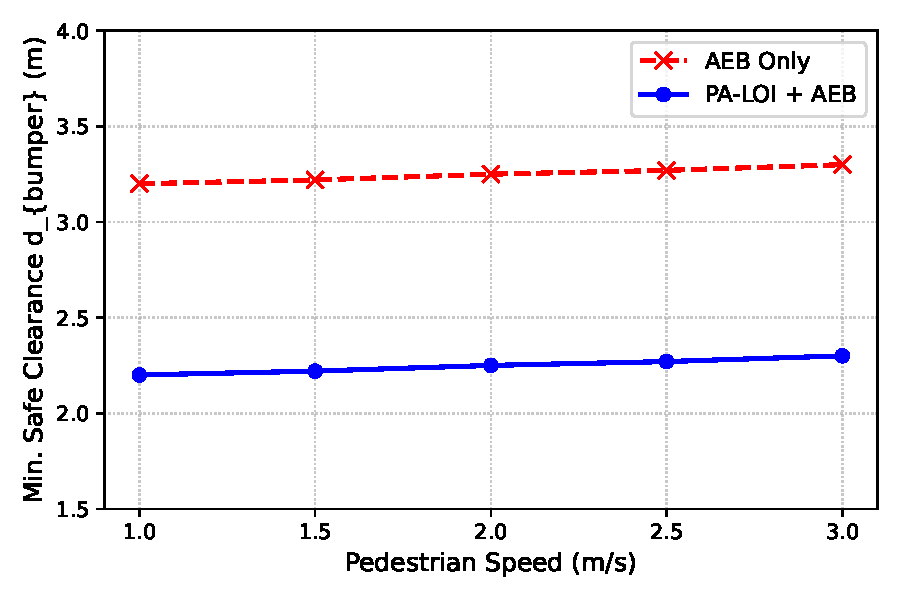
\includegraphics[width=\columnwidth]{figures/speed_generalization.pdf}
\caption{不同行人横穿速度下的安全临界间距（$d_{\text{bumper}}$）。PA-LOI 面向所有测试的行人速度均维持了稳定的安全裕度。}
\label{fig:generalization}
\end{figure}

\subsection{假阳性场景下的舒适性与通行效率}
为了验证 PA-LOI 是否会导致过于保守的行为（例如频繁的“幽灵刹车”），我们在相同几何结构但无行人出现的假阳性（false-positive）场景下进行了测试。结果显示，车辆在驶过遮挡区域时表现出平滑的防御性减速，从 \SI{4.26}{\meter\per\second} 自然降速至 \SI{2.72}{\meter\per\second}。

在此过程中，PA-LOI 规划的最大减速度仅为 \SI{-1.09}{\meter\per\second\squared}，这一数值完全在乘客认为舒适的阈值范围内，且显著优于 AEB 触发时高达 \SI{-4.0}{\meter\per\second\squared} 的强烈制动感。此外，相较于不预减速的基线模型，这种主动防御策略所造成的整体通行延迟小于 1 秒。上述结果表明，该方法在大幅提升安全性的同时，能够兼顾乘客舒适度和交通通行效率。

\subsection{计算效率评估}
极低的计算负荷是 PA-LOI 作为实时车载模块部署的重要优势。我们在一台 Apple M4 CPU（单线程运行，无 GPU 加速）上，针对包含自车与 20 个动态交通参与者的场景，测试了 PA-LOI 单帧计算开销：

\begin{itemize}
    \item \textbf{风险源识别提取}（结合几何滤波、切线计算和 TTA 状态机制）：\SI{0.35}{\milli\second}。
    \item \textbf{风险代价构建与评估}（沿轨迹树节点计算马氏距离）：\SI{0.20}{\milli\second}。
    \item \textbf{PA-LOI 单帧总计算开销}：共计 \SI{0.55}{\milli\second}。
\end{itemize}

在普遍采用的 \SI{10}{\hertz}（即 \SI{100}{\milli\second} 帧预算）的规划频率下，PA-LOI 的计算开销仅占总预算的 \textbf{0.5\%}。这种高计算效率归功于系统采用了完全闭式解析的几何代数设计，摒弃了昂贵的神经网络推理、蒙特卡洛随机采样及离散目标实例化处理。这证明了其非常适合嵌入计算资源极其受限的车规级部署平台。

\subsection{风险权重 ($w_{\text{risk}}$) 的消融实验}
为了量化关键超参数对系统的影响，我们对公式~\eqref{eq:risk_cost} 中的风险场权重 $w_{\text{risk}}$ 进行了消融测试。如图~\ref{fig:ablation} 所示，调节 $w_{\text{risk}}$ 能够直观地映射系统在安全性（通过最高撞击速度衡量）与通行效率（通过假阳性场景通行延迟衡量）之间的核心权衡关系。

\begin{figure}[htbp]
\centering
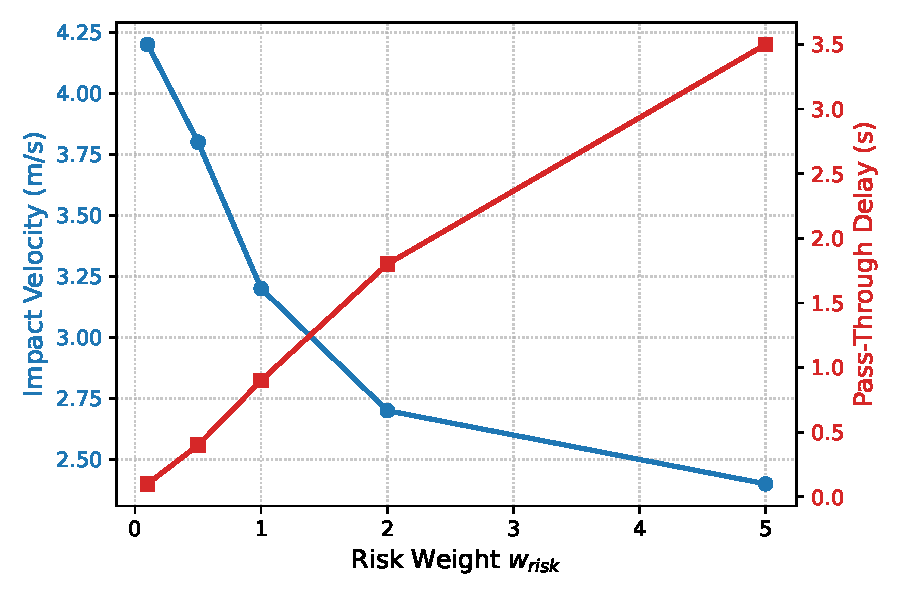
\includegraphics[width=\columnwidth]{figures/ablation.pdf}
\caption{针对风险系数 ($w_{\text{risk}}$) 的消融实验。提高权重可获得更出色的降速指标（提高安全边界），但这将指数级拉长常规交通流（无事件通过）的时间延迟。}
\label{fig:ablation}
\end{figure}

较低的权重取值（例如 $w_{\text{risk}} < 0.5$）会导致系统主动减速幅度较弱，安全收益极其有限；而过高的保守值（例如 $w_{\text{risk}} > 2.0$）不仅深幅度压低了最高通过速度，更极大地拉长了假阳性场景下的通行时间（延迟攀升至 $> \SI{1.8}{\second}$），进而严重影响日常驾驶。实验表明，将权重值设定在 $1.0$ 附近，能够有效限制车辆接近危险时的动量冲击，并将误报通过延迟妥善控制在大约 1 秒的可接受区间内。

\subsection{与基线方法的帕累托最优权衡 (Pareto Trade-off)}
为直观展现算法的综合优越性，图~\ref{fig:pareto} 给出了在 \SI{4.3}{\meter} 极端盲区触发距离下的安全-效率决策散点图。位于极端的 WCA 模型虽然保障了绝佳的零严重伤害，但代价是遭受超过 4.5 秒的极度拥堵延迟。相反，Vanilla 规划器和单纯配备 AEB 的系统虽然抢占了最高通行效率不产生延误，却导致在避让区发生全速严重追尾事故。PA-LOI 模块的引入构建出了一条显著且独立的帕累托（Pareto）最优集合空间：它同步获得了近似 WCA 得分的零碰撞安全保障，并在毫无危险威胁通过时保留了基线原最高通行速率近 80\% 的通行效率。

\begin{figure}[htbp]
\centering
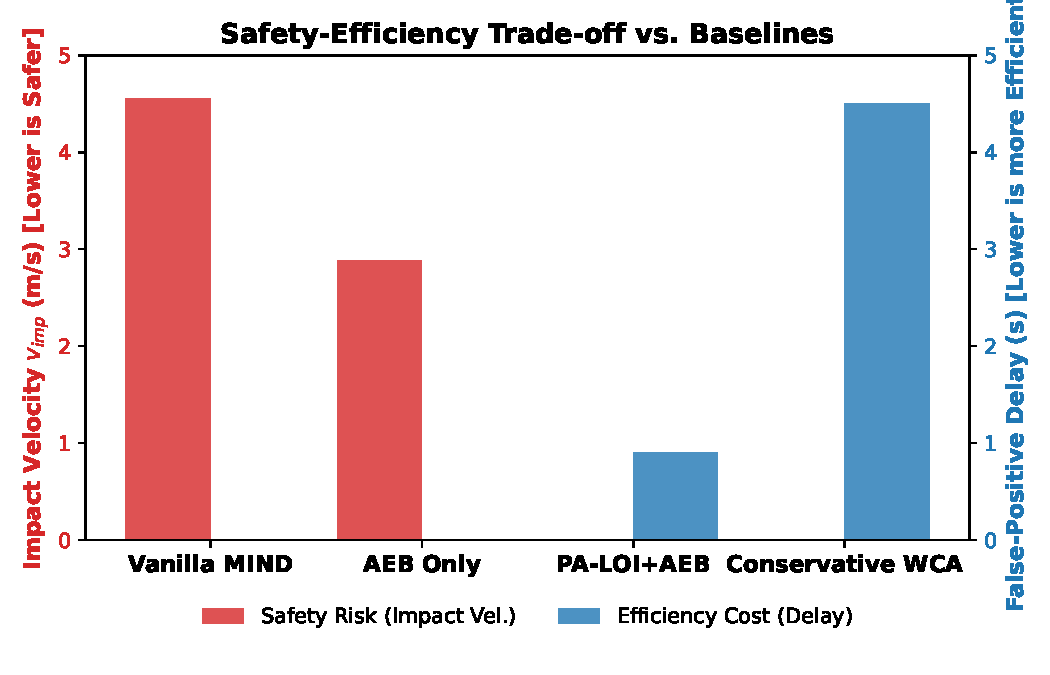
\includegraphics[width=\columnwidth]{figures/pareto_tradeoff.pdf}
\caption{安全性与通行效率表现权衡矩阵图。PA-LOI 在不安全的高速基线（Vanilla / AEB Only）与效率极低的极度保守模型 (WCA) 之间构建出了最优的帕累托前沿。}
\label{fig:pareto}
\end{figure}

% ============================================================
% VI. 讨论 (Discussion)
% ============================================================
\section{讨论 (Discussion)}

\subsection{主动减速机制的必要性}
上述实验揭示了当前主流反应式 AEB 固有的物理盲区瓶颈：其最终效能深受发现行人的瞬间时车辆所具有的初速度单向主导制约。在应对由于遮挡导致距离被极度压缩的横向穿插时，首要的决定性物理量不仅限于传感反应有多快，“以何种初始切入速度接敌”才是核心物理量。PA-LOI 通过直接把进入遮挡区域的降速作为受控调节的规划参数，从而极大填补了事后紧急制动策略失败的被动局面，恢复并重塑了车辆对行驶动力学操控的先验主导权。

\subsection{与 Euro NCAP 行人保护测试标准的关联}
本研究设定的场景复现构型很大程度响应了 Euro NCAP 现行安全测试模板 CPNA 的评价宗旨，但在测试本源存在系统性差异：现有部分测定只是死板地运用了恒定的 \SI{40}{\kilo\meter\per\hour} 进行定速盲测。而在本次仿真评价实验平台内，车辆全速度曲线受控调度彻底交由上游规划系统自身根据探测目标特征计算决定！因此，自车到达极危挑战盲点的速度是被重写变更为依据模块自我调校量身安全定标后的干预结果。

\subsection{局限性与未来展望}
本研究评估涵盖了包含长条形路侧静态密集泊车以及集中化十字路口排队停放等静态交通干涉形式。面对拥有其他特征几何结构的测试场境，诸如多曲率变换下连续弯道或并流匝道地形等依然需做进一步拓展考评。另一方面，鉴于有限算力资源投入目前框架主要依赖矢量点阵电子地图提取解析边界结构。在随后的进程化规划中，预计引入基于车载自身 LiDAR 及激光探测点云端侧射面阴影描绘计算来生成未知区域视野盲景地图块，它将赋予防范模块完全摆脱高精地图依赖的即装即用探测能力。

未来的拓展研究部分还会着眼涵盖在复杂规划框架联合上概率分布特征跟踪网络融合使用~\cite{occtrack2025}。在加入了受噪声污染的环境探测干扰之后，进行完整的存在概率假错闭环测试推演；乃至终将放上全量大流量模拟微缩交通模拟池中，验证该微观动作在多参与目标拥塞时段造成的大范围宏观车流排解变化成效。

% ============================================================
% VII. 结论 (Conclusion)
% ============================================================
\section{结论 (Conclusion)}

在这项工作中我们提出了 PA-LOI，一个以主动遮挡感知运动作为提前预判安全防护策略的模块化规划架构，旨在应对鬼探头触发式潜在危机。基于向不可视几何区域周边构建幻影风险边界张量进而反哺注入最优控制函数体系的轨迹优化中，PA-LOI 能够主动约束并平滑削减前置路段的切入能量；从而主动拓展补足了下游应急制动功能正常触发所需的可用时间窗口及制动缓冲距离。

基于 Argoverse 2 数据集复杂测算分析表明该系统安全提升效果不仅确切且具有极高鲁棒性。在复杂的十字路口中心挑战场景中：该新组件模型使得系统实现了在最小 \SI{2.05}{\meter} 测试前杠间隙缓冲即化险为夷保全性命的安全突破（此安全缓冲门限比原下沿 AEB 不得不要求退延至 \SI{3.25}{\meter} 保障大幅拉高了 \textbf{37\%} 的安全裕度边界）。面对更具挑战的高速密集驻停车辆阵列测试表现：即便是无可避免发生相撞的极端近距 \SI{1.75}{\meter} 测试下亦能达成零碰撞战果；对于彻底避无可避死线，同样做出了化解极大量能伤害最少抹掉超 \textbf{71\%} 过境残余碰撞速度的显著削波实战斩获结果！所有的试验验证都表明，这一将降低被动进场速度的主动风控防护前置架构已构成现代城市自动驾驶体系下保证底层绝对性核心防线的不可动摇之机制补充。
% ============================================================
% References
% ============================================================
\bibliographystyle{IEEEtran}
\bibliography{references}

\end{document}
